\section{Eating on La Vigilia}


It has been a tradition in our family, both the Sicilian and Abruzzesi sides, to have a seafood dinner on Christmas Eve. It starts with an antipasto that includes tuna and anchovy, and ends with an assortment of smelts, shrimp, and baccalà. But as the family dispersed and the number of guests decreased, so did the assortment of seafood.

\paragraph{Primo Piatto}


In any case, my favorite has always been the first plate and is actually all that I need to consider the dinner complete. This is calamari sauce. It is simple to make, so I am providing the recipe here in case you have not yet made your Christmas Eve plans.

\subparagraph{Prepare the Sauce}


\begin{enumerate}


\item Heat olive oil in a sauce pan, and sauté some finely chopped onions.

\item Optional: include some diced yellow onion if you prefer it.

\item Add salt and pepper to taste; I don't like too much salt.

\item When onions and garlic is ready add tomato puree. I use Pomi strained tomatoes which comes in 750 g boxes. Two boxes minimum or three or even more for more people or hearty eaters.

\item I like to add a bottle of clam juice and/or dry Marsala; perhaps white wine if you have it around.

\item Let it all simmer slowly for a while.
\end{enumerate}


\subparagraph{Get the seafood ready}


Slice up some squid in rings and don't be shy about including the tentacles, which are the tastiest part. A giant squid would have no compunction about eating you.

Add the squid to the sauce and let them cook. Not too long so they don't get tough. That suffices if that is all you want to do.

I like to include some mussels and/or claims. Brush the shells clean and add them several minutes before serving. You need to wait for the shells to open.

You can even add some pealed and deveined shrimp. If I have enough sauce I add a lobster tail for special occasions.

\subparagraph{Serving the meal}


\begin{wrapfigure}{rt}{.3\textwidth}
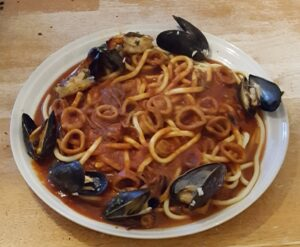
\includegraphics[width=.3\textwidth]{Calamari_quarter-300x247.jpg}
\end{wrapfigure}

Cook some pasta, following package directions id you don't already know how. I prefer past with more body like linguini, although my absolute favorite is bucatini. It is easy to cook al dente and the sauce penetrates the entire strand. When the pasta is ready, transfer it to a serving bowl and cover it with the sauce. Always include extra sauce at the table.


Purists insist that you should never serve cheese with a seafood sauce. However, my family has always used grated pecorino romano cheese quite liberally on the pasta.

I know that because my job was always to grate the cheese.

\paragraph{Dining in~Castellammare}

\begin{wrapfigure}{rt}{.3\textwidth}
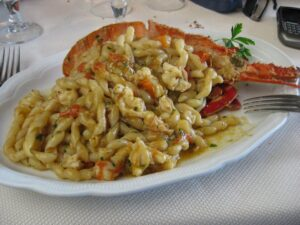
\includegraphics[width=.3\textwidth]{LobsterInSicily-300x225.jpg}
\end{wrapfigure}

This is a postscript, demonstrating how to be creative with your cooking. About 10 years ago, my son and I were touring around Sicily. On one trip to Castellammare, we saw a restaurant displaying all the fresh seafood at the entrance. So we found a table. Just as we were deciding what to order, a small truck stopped and unloaded fresh seafood that was place immediately in the display case.

We got up to check it out and saw a beautiful lobster, which we ordered. The waiter then enquired about how we would like it prepared. We looked a little puzzled. Noticing that, the waiter said, ``Don't worry! I'll make something nice for you.'' A short time later, he returned with this beautiful and delicious dish. And, yes, he offered us some grated cheese to cover it.


\flrightit{Posted on 2021-12-18 by Cologero}

\begin{center}* * *\end{center}

\begin{footnotesize}
\begin{sffamily}
\texttt{Oswald Spengler on 2021-12-19 at 02:46 said:}

What a great recipe. This website is worth reading if only for Cologero's Italian cuisine instructions. I can't cook to save my life but wow, Cologero really makes me want an Italian wife who'd cook me these kinds of dishes

\hfill

\texttt{Balder on 2021-12-19 at 11:45 said:}

Being a Finn, I prefer overcooked ham with rye bread and mustard, salmon with potatoes and liver \& carrot casserole on the Yule table. Being thinking also turning full vegetarian, but I will never touch that horrible seitan.

\hfill

\texttt{Auld Wat on 2021-12-20 at 13:38 said:}

I will be fasting on the Vigil. So sadly while I can see the food, I can't eat it.

\hfill

\texttt{Cassiodorus on 2022-12-20 at 12:29 said:}

As a fellow Italian American , I totally appreciated this post . When I was a kid , the big fish dinner wasn't a winner . Later on , when I came to enjoy seafood , the Christmas Eve feast is something I look foreword to all year.

Grazie Mille !

\end{sffamily}
\end{footnotesize}

